\section{Auswertung}
\label{sec:Auswertung}


Die Graphen wurden sowohl mit Matplotlib \cite{matplotlib} als auch NumPy \cite{numpy} erstellt. Die
Fehlerrechnung wurde mithilfe von Uncertainties \cite{uncertainties} durchgeführt.

\subsection{Apparatekonstanten}
Für die Messreihen wurde Gerät 2 verwendet.
Die Werte für Induktivität $L$ der Spule, die Kapazität $C$ und den verwendeten Widerstand $R_.1$ befinden sich in Tabelle \ref{tab:tab1}

\begin{table}
	\centering
	\caption{Apparatekonstanten}
\label{tab:tab1}
	\sisetup{table-format=1.2}
	\begin{tabular}{S[table-format=1.2]S[table-format=1.3]S[table-format=2.1]}
		\toprule
		{$L/ 10^3 \si{\hertz}$} & {$C/10^9\si{\farad}$} & {$R/\si{hertz}$} \\
		\midrule
		${10,11\pm 0,03}$ & ${2,098\pm 0,006}$ & ${48,1\pm 0,1}$ \\
		\bottomrule
	\end{tabular}
\end{table}
\subsection{Abklingzeit und effektiver Dämpfungswiderstand}
In Tabelle \ref{tab:tab2} sind die Messwerte des in Abbildung \ref{fig:abb1} sichtbaren Graphen zu sehen.\newline
Als Generatorspannung wurde eine Rechteckspannung von $U_.G=20V$ verwendet.
\begin{table}
	\centering
	\caption{Apparatekonstanten}
\label{tab:tab2}
	\sisetup{table-format=1.2}
	\begin{tabular}{S[table-format=3.0]S[table-format=2.1]}
		\toprule
		{$t/10^{-6}\si{\second}$} & {$U_.C/\si{\volt}$} \\
		\midrule
		0 & 19.4 \\
		30 & 16.0 \\
		60 & 13.4 \\
		90 & 11.2 \\
		120 & 9.6 \\
		150 & 8.0 \\
		180 & 7.0 \\
		210 & 5.8 \\
		240 & 4.8 \\
		270 & 4.0 \\
		300 & 3.6 \\
		330 & 3.0 \\
		360 & 2.6 \\
		390 & 2.2 \\

		\bottomrule
	\end{tabular}
\end{table}
\begin{figure}
\centering
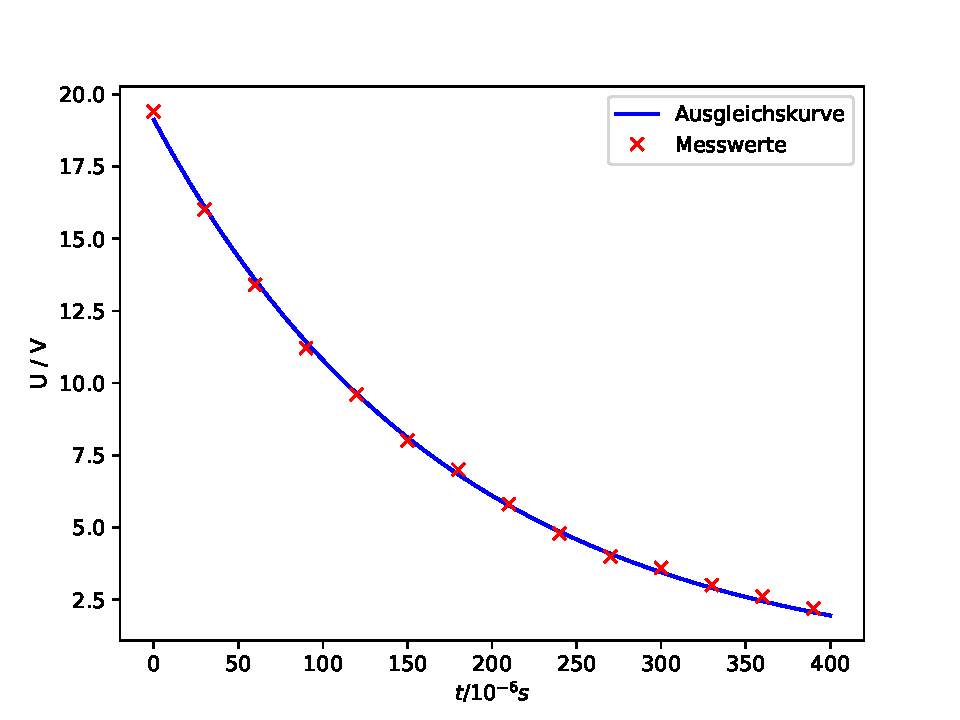
\includegraphics[scale=0.6]{content/images/a.pdf}
\caption{Messdaten eines Abklingvorgangs eines RLC-Schwingkreises}
\label{fig:abb1}
\end{figure}
\newpage
\noindent Die Regression $U(t)=A_.0e^{-2\pi\mu t}$ liefert:
\begin{align}
A_.0 &= \SI{19,11(12)}{\volt} \\
\mu &= \SI{909(9)}{\hertz}
\end{align}
Nach Gleichung \eqref{eq:gamma} und \eqref{eq:tau} ergibt sich mit $\gamma=2\pi\mu$:
\begin{align}
R_.{eff}&=\SI{115(1)}{\ohm} \\
\tau &=\SI{175(1)e-6}{\second}
\end{align}
Der Fehler von $R_.{eff}$ errechnet sich dabei aus der Gaußschen Fehlerfortpflanzung
\[
\sigma_.R=\sqrt{(4\pi L\sigma_.{\mu})^2 +(4\pi\mu\sigma_.L)^2)},
\]
wobei $\sigma_.L$ aus Tabelle \ref{tab:tab1} abzulesen und $\sigma_.{\mu}$ durch die Regression bestimmt wurde.
Analog dazu errechnet sich der Fehler der Abklingzeit $\tau$ zu
\[
\sigma_.{\tau}=\frac{\sigma_.{\mu}}{2\pi\mu^2}
\]
Der berechnete effektive Widerstand $R_.{eff}$ weicht von dem geschalteten Widerstand $R_.1$ um $\Delta R=140\%$ ab.
\subsection{Aperiodischer Grenzfall}
Der Widerstand für den die Schwingung in den aperiodischen Grenzfall übergeht wurde zu
\[
R_.{ap,exp}=\SI{3,5e3}{\ohm}\text{.}
\]
Der aus Gleichung \eqref{eq:} berechnete Wert beträgt
\[
R_.{ap,theo}=\SI{4,390(9)e3}{\ohm},
\]
wobei sich der Fehler aus
\[
\sigma_.{R}=\sqrt(\sigma_.L^2/(CL)+(L\sigma_.C)^2/(C^3L))
\]
berechnet.\newline
Die Abweichung beträgt somit
\[
\Delta R_.{ap}=25,4\%
\]
\subsection{Frequenzabhängigkeit der Kondensatorspannung}
\subsubsection{Frequenzabhängigkeit der Amplitude}
Die in Tabelle \ref{tab:tab3} festgehaltenen Werte der eingestellten Frequenz $\nu$ und der gemessenen Kondensatorspannung $U_.C$ sowie ihres Verhältnisses zur Generatorspannung $U_.G=\SI{9,8}{\volt}$
wurden in Abbildung \ref{fig:abb2} halblogarithmisch gegeneinander aufgetragen.\newline
In Abbildung \ref{fig:abb3} wurde der Ausschnitt um die Resonanzfrequenz herum linear dargestellt, um die Schärfe $\nu_.+-\nu_.-$ der Frequenz zu bestimmen.
\begin{table}
	\centering
	\caption{Messwerte zur Frequenzabhängigkeit der Kondensatorspannung}
\label{tab:tab3}
	\sisetup{table-format=1.2}
	\begin{tabular}{S[table-format=2.1]S[table-format=3.1]S[table-format=2.2]}
		\toprule
		{$\omega/10^3\si{\second}$} & {$U_.C/\si{\volt}$} & {$\frac{U_.C}{U_.G}/\si{}$}\\
		\midrule
		15 & 12.2 & 1.24 \\
		20 & 15.0 & 1.53 \\
		25 & 21.6 & 2.20 \\
		30 & 47.2 & 4.82 \\
		31 & 63.2 & 6.45 \\
		32 & 95.2 & 9.71 \\
		32.5 & 122 & 12.45 \\
		33 & 150 & 15.31 \\
		33.3 & 157 & 16.02 \\
		33.6 & 150 & 15.31 \\
		34.1 & 122 & 12.45 \\
		34.6 & 96.8 & 9.88 \\
		35.6 & 63.2 & 6.45 \\
		36.6 & 45.6 & 4.65 \\
		41.6 & 17.4 & 1.78 \\
		46.6 & 10.4 & 1.06 \\
		50 & 8.0 & 0.82 \\
		\bottomrule
	\end{tabular}
\end{table}
\begin{figure}
\centering
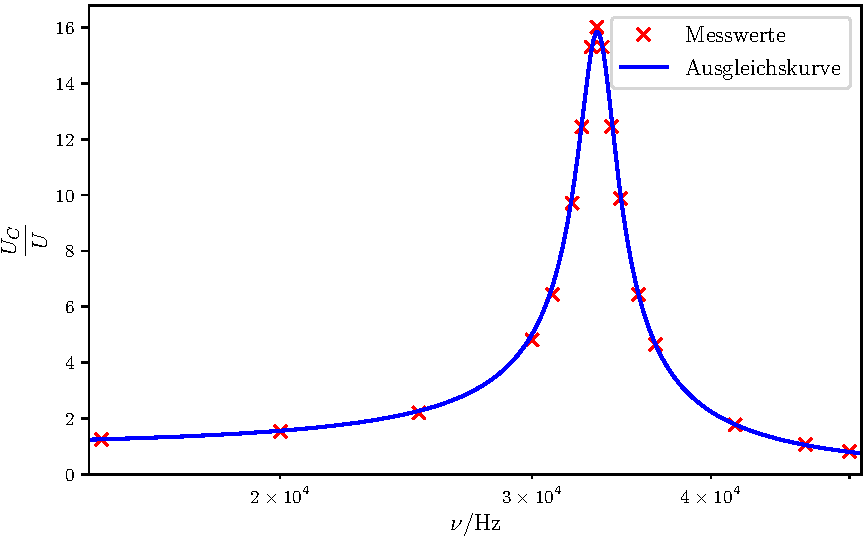
\includegraphics[scale=0.8]{content/images/Graphc1.pdf}
\caption{halblogarithmische Darstellung des Spannungsverhältnisses $\frac{U_.C}{U_.G}$ in Abhängigkeit von der Frequenz $\nu$}\label{fig:abb2}
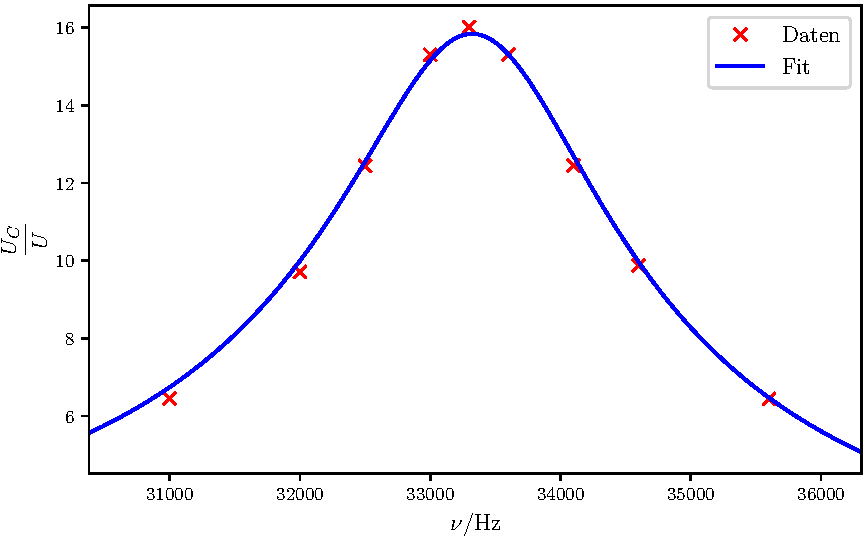
\includegraphics[scale=0.8]{content/images/Graphc2.pdf}
\caption{Lineare Darstellung in der Nähe der Resonanzfrequenz}
\label{fig:abb3}
\end{figure}
\newpage
\noindent
Die gemessene Güte $q_.{exp}$ lässt sich leicht aus Tabelle \ref{tab:tab3} ablesen:
\[
q_.{exp}=16,02
\]
Aus Gleichung \eqref{eq:} lässt sich die theoretische Güte 
\[
q_.{theo}=19,0\pm 0,2
\] berechnen.
Der Fehler ist dabei durch 
\[
\sigma_.q=\sqrt{\frac{\sigma_.R^2L}{CR^4}+\frac{\sigma_.C^2L^2}{C^34R^2L}+\frac{\sigma_.L^2}{4R^2CL}}
\]
gegeben.
Die Abweichung zwischen Theorie und Experiment beträgt
\[
\Delta q = 18,65\%
\]
Die gemessene Breite der Resonanzkurve ergibt sich mit $\nu_.-=$ und $\nu_.+=$:
\[
(\nu_.+-\nu_.-)_.{exp}=\SI{}{\hertz}
\]
Der aus Gleichung \eqref{eq:} berechnete beträgt
\[
(\nu_.+-\nu_.-)_.{theo}=\SI{11,42(12)e3}{\hertz}\text{.}
\]
Der Fehler berechnet sich über
\[
\sigma_.{\nu_.+-\nu_.-}=\sqrt{\frac{\sigma_.R^2}{L^2}+\frac{R^2\sigma_.L^2}{L^4}}
\]
\subsubsection{Frequenzabhängigkeit der Phase}
Die Werte des in Abbildung \ref{fig:abb4} und \ref{fig:abb5} sichtbaren Graphen lassen sich aus Tabelle \ref{tab:tab4} ablesen.
\begin{table}
	\centering
	\caption{Messwerte zur Frequenzabhängigkeit der Kondensatorspannung}
\label{tab:tab4}
	\sisetup{table-format=1.2}
	\begin{tabular}{S[table-format=2.1]S[table-format=2.1]S[table-format=3.2]}
		\toprule
		{$\omega/10^3\si{\second}$} & {$a/10^{-6}\si{\second}$} & {$\phi/\si{\degree}$}\\
		\midrule
		15 & 0,6 & 3,24 \\
		20 & 0,6 & 4,32 \\
		25 & 0,6 & 5,40 \\
		30 & 1,0 & 10,80 \\
		31 & 1,2 & 13,39 \\
		32 & 2,2 & 25,34 \\
		32.5 & 3,0 & 35,10 \\
		33 & 5,0 & 59,40 \\
		33.3 & 7,2 & 86,31 \\
		33.6 & 9,2 & 111,28 \\
		34.1 & 11,2 & 137,49 \\
		34.6 & 12,4 & 154,45 \\
		35.6 & 13,0 & 166,61 \\
		36.6 & 13,0 & 171,29 \\
		41.6 & 11,6 & 173,72 \\
		46.6 & 10,6 & 177,82 \\
		50 & 9,8 & 176,40 \\
		\bottomrule
	\end{tabular}
\end{table}
\begin{figure}
\centering
%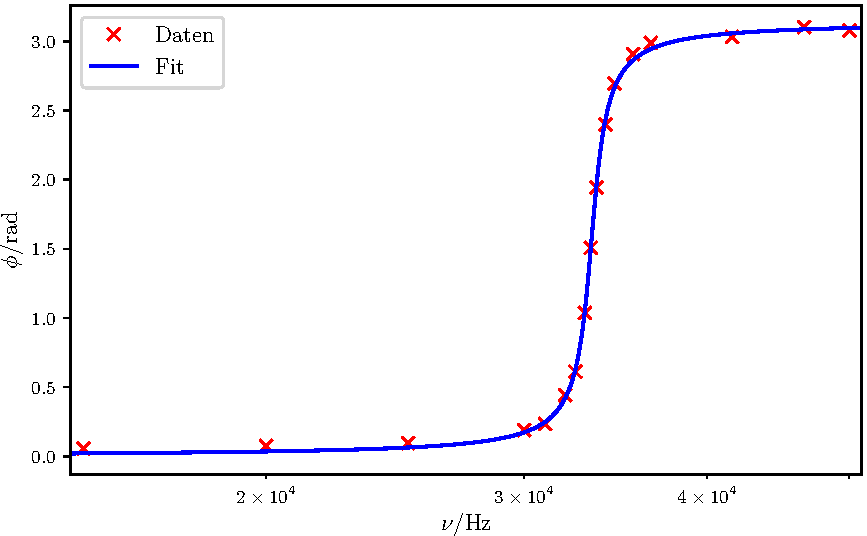
\includegraphics[scale=0.8]{content/images/Graphd1.pdf}
\caption{Verlauf der Phasenverschiebung in Abhängigkeit von der Frequenz}
\label{fig:abb4}
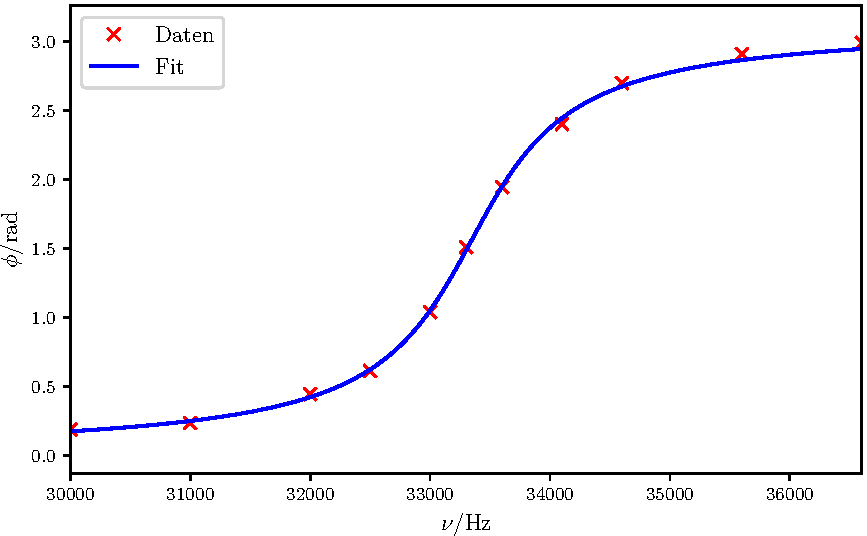
\includegraphics[scale=0.8]{content/images/Graphd2.pdf}
\caption{Verlauf der Phasenverschiebung in der Nähe der Resonanzfrequenz}
\end{figure}